\documentclass[11pt]{article}
\usepackage[paper=a4paper, top=25mm, bottom=20mm, textwidth=5.8in]{geometry}

% Font and encoding
\usepackage{lmodern}           % Better Computer Modern font
\usepackage[T1]{fontenc}       % Better glyph encoding
\usepackage[utf8]{inputenc}    % Necessary for unicode characters
\usepackage[english]{babel}    % Necessary for correct hyphenation
\usepackage{textcomp}          % Necessary to display unicode characters like €
\usepackage{csquotes}          % Quotation marks (\MakeOuterQuote{"} needed)
\usepackage{microtype}         % Avoid unnecessary overfull / underfull hboxes

% Other packages
\usepackage[style=authoryear]{biblatex}    % Bibliography
\usepackage[parfill]{parskip}              % Add space between paragraphs
\usepackage[hidelinks]{hyperref}           % Clickable \ref and \cite
\usepackage{graphicx}                      % Needed for figures
\usepackage{booktabs}                      % Needed for tables
\usepackage{caption}                       % Needed for captionsetup
\usepackage{subcaption}                    % Needed for subfigure and subtable
\usepackage{amsmath}                       % Better math environments and \text
\usepackage{physics}                       % e.g. for derivative formatting
\usepackage{siunitx}                       % \si{\unit} and \SI{value}{\unit}
\usepackage{titlesec}                      % Needed for titleformat
\usepackage{authblk}                       % Authors formatting
\usepackage{tablefootnote}

\usepackage{xcolor}
\newcommand{\DEVELOPMENT}{1} % 1= show comments, 0=no comments
\usepackage{ifthen}
\ifthenelse{\DEVELOPMENT = 1}{
	\newcommand{\tz}[1]{\textcolor{red}{\textbf{TZ:} #1}}		
	\renewcommand{\oe}[1]{\textcolor{magenta}{\textbf{OE:} #1}}
}{
\newcommand{\tz}[1]{}
\renewcommand{\oe}[1]{}
}

% Setup
\MakeOuterQuote{"}
\setlength\parindent{0pt}
\captionsetup{width=.9\linewidth}

\addbibresource{bib.bib}

\title{Effects of Layer Freezing when Transferring\\DeepSpeech to New Languages}
\author[1]{\textbf{Onno Eberhard}}
\author[ ]{\textbf{Torsten Zesch}}
\affil[ ]{Language Technology Lab}
\affil[ ]{University of Duisburg-Essen}
\affil[1]{\href{mailto:onno.eberhard@stud.uni-due.de}{\texttt{onno.eberhard@stud.uni-due.de}}}
\date{}

\begin{document}
\maketitle

\begin{abstract}\noindent
In this paper, we train Mozilla's DeepSpeech architecture on German and Swiss German speech datasets and compare the results of different training methods. We first train the models from scratch on both languages and then improve upon the results by using an English pretrained version of DeepSpeech for weight initialization and experiment with the effects of freezing different layers during training. We see that even freezing only one layer already improves the results dramatically.
%We build on previous efforts by \textcite{agarwal-zesch-2019-german} and reproduce their results by training the model from scratch. We improve upon these results by using an English pretrained version of DeepSpeech for weight initialization and experiment with the effects of freezing different layers during training. We see that freezing even one layer already improves the results dramatically.
\end{abstract}

\section{Introduction}
The field of automatic speech recognition (ASR) is dominated by research specific to the English language. There exist plenty available text-to-speech models pretrained on (and optimized for) English data. When it comes to a low-resource language like Swiss German, or even standard German, the range of available pretrained models becomes very sparse. In this paper, we train Mozilla's implementation\footnote{\url{https://github.com/mozilla/DeepSpeech}} of Baidu's DeepSpeech ASR architecture \parencite{hannun2014deep} on these two languages. We use transfer learning to leverage the availability of a pretrained English version of DeepSpeech and observe the difference made by freezing different numbers of layers during training.

For previous work on using DeepSpeech for the two languages German and Swiss German, see \parencite{agarwal-zesch-2019-german} and \parencite{agarwal2020ltl} respectively. Note however, that our datasets and training methods are not identical to those used there. Our focus here lies on isolating the effect of layer freezing in the given context.

\section{Transfer Learning and Layer Freezing}
Deep neural networks can excel at many different tasks, but they often require very large amounts of training data and computational resources. To remedy this, it is often advantageous to employ transfer learning: Instead of initializing the parameters of the network randomly, the optimized parameters of a network trained on a similar task are reused. Those parameters can then be fine-tuned to the specific task on hand, using less data and fewer computational resources. In the fine-tuning process many parameters of the original model may be "frozen", i.e. held constant during training. This can speed up training, as well as decrease the computational resources used during training \parencite{DBLP:conf/rep4nlp/KunzeKKKJS17}. The idea of taking deep neural networks trained on large datasets and fine-tuning them on tasks with less available training data has been popular in computer vision for years \parencite{huh2016makes}. More recently, with the emergence of end-to-end deep neural networks for automatic speech recognition (like DeepSpeech), it has also been used in this area \parencite{DBLP:conf/rep4nlp/KunzeKKKJS17, DBLP:journals/corr/abs-1911-09271}.

The reason why the freezing of parameters for fine-tuning deep neural networks is so successful, is that the networks learn representations of the input data in a hierarchical manner. The input is transformed into simplistic features in the first layers of a neural network and into more complex features in the layers closer to the output. With networks for image classification this can be nicely visualized \parencite{10.1007/978-3-319-10590-1_53}. As for automatic speech recognition, the representations learned by the layers of a similar system to the one we used, one that is also based on Baidu's DeepSpeech architecture, have been analyzed by \textcite{NIPS2017}. The findings show that the hierarchical structure of features learned by DeepSpeech is not as clear as it is with networks for image processing. Nonetheless, some findings, for example that affricates are better represented at later layers in the network, seem to affirm the hypothesis that the later layers learn more abstract features and earlier layers learn more primitive features. This is important for fine-tuning, because it only makes sense to freeze parameters if they don't need to be adjusted for the new task. If it is known that the first layers of a network learn to identify "lower-level"-features, i.e. simple shapes in the context of image processing or simple sounds in the context of ASR, these layers can be frozen completely during fine-tuning.

The DeepSpeech network takes features extracted from raw audio data as input and outputs character probabilities (the architecture is described in more detail in the next section). With the reasoning from above, the first few layers should mostly obtain simple features, such as phonemes, from the input, while the later layers should mostly infer the character corresponding to these lower level features. The rationale for using transfer learning to transfer from one language to another, is the assumption that these lower-level features are shared across different languages. Thus, only the parameters later layers need to be adjusted for successfully training the network on a new language. Whether this assumption works in practice, and how much use freezing the layers actually is, will be the focus of this paper. We train the English pretrained version of DeepSpeech on German and on Swiss German data and observe the impact of freezing fewer or more layers during training.
%
% The rationale for using transfer learning is not only that English and German are closely related languages. In fact, one could argue that they are very different in this context, because DeepSpeech is trained to directly infer written characters from audio data and English and German pronunciations of some characters differ greatly. However, the first few layers of the DeepSpeech network are likely not inferring the final output character, but rather lower level features of the spoken input, such as phonemes, which are shared across different languages. Thus, this approach should also work for languages which are not related at all. It is to be expected that the model should give better results when trained on a small dataset than a model trained from scratch, because it does not have to learn these lower level features again.
%
%
% In most applications where fine-tuning is employed, it is a safe assumption
%
%
% -> CNN visualization paper
% imagenet / layer freezing paper
% Für das ähnliche Modell DeepSpeech2 werden die gelernten repräsentationen in (NIPS17) untersucht
%
% An sich sind die ersten layers = lower-level-features -> Simple shapes bei Vision, simple sounds bei asr.
% Sollten sich nicht großartig unterscheiden zwischen verschiedenen sprachen (mit nächstem absatz verbinden)
% trotzdem noch zeigen, wo -transfer learning- in ASR benutzt wurde (Ruder)
% wenn keine analysis zu verschiedenen layers gefrozen zu finden ist dann ist das halt so
%
% In this work, we want to explore what the benefits 
%
% \tz{some theory on layer freezing and where this has been successfully used before}

\section{Experimental Setup}
%\tz{ich habe versucht das aufzuteilen aber Struktur der Untersections passt noch nicht ganz}
\subsection{DeepSpeech architecture}
We use Mozilla's DeepSpeech version 0.7 for our experiments. The implementation differs in many ways from the original model presented by \textcite{hannun2014deep}. The architecture is described in detail in the official documentation\footnote{\url{https://deepspeech.readthedocs.io/en/latest/DeepSpeech.html}} and is depicted in Figure~\ref{fig:ds}. From the raw speech data, Mel-Frequency Cepstral Coefficients \parencite{imai1983cepstral} are extracted and passed to a 6-layer deep recurrent neural network. The first three layers are fully connected with a ReLU activation function. The fourth layer is a Long Short-Term Memory unit \parencite{hochreiter1997long}; the fifth layer is again fully connected and ReLU activated. The last layer outputs probabilities for each character in the language's alphabet. It is fully connected and uses a softmax activation for normalization. The character-probabilities are used to calculate a Connectionist Temporal Classification (CTC) loss function \parencite{graves2006connectionist}. The weights of the model are optimized using the Adam method \parencite{kingma2014adam} with respect to the CTC loss.

\begin{figure}[ht]
    \centering
    \includegraphics[width=.85\textwidth]{ds.png}
    \caption{DeepSpeech architecture (adapted from the official documentation\protect\footnotemark[\value{footnote}])}
    \label{fig:ds}
\end{figure}

\subsection{Training Details} \label{sec:training}
To assess the effects of layer freezing, we train the network multiple times for each of the two languages. For weight initialization we use an English pretrained model, which is provided by Mozilla\footnote{\url{https://github.com/mozilla/DeepSpeech/releases}}. We then freeze between 0 and 4 layers during training. For both languages we also train one model from scratch, where the weights are initialized randomly. In total, we train 6 different models for each language:
\begin{description}
    \item[Reference] The whole model from scratch (random weight initialization)
    \item[0 Frozen Layers] The model with weights initialized to those of the English pretrained model, all weights are optimized during training
    \item[1 Frozen Layer] The English-initialized model with the first layer frozen
    \item[2 Frozen Layers] The English-initialized model with the first two layers frozen
    \item[3 Frozen Layers] The English-initialized model with the first three layers frozen
    \item[4 Frozen Layers] The English-initialized model with the first three and the fifth layer frozen
\end{description}
%\paragraph{Layer Freezing}
%We used Mozilla's DeepSpeech version 0.7.4 for training the model from scratch and version 0.7.3 for the transfer learning approach. 
%\tz{warum der Unterschied?}
The complete training script, as well as the modified versions of DeepSpeech that utilize layer freezing are available online\footnote{\url{https://github.com/onnoeberhard/deepspeech-paper}}.
The weights were frozen by adding \texttt{trainable=False} at the appropriate places in the TensorFlow code. For all models, we had to reinitialize the last layer, because of the different alphabet sizes of German / Swiss German and English (ä, ö, ü).
%In transfer learning, all weights of the model are initialized to those of the . In addition to transfer learning, we also train the model from scratch with random weight initialization, thereby reproducing a result from \textcite{agarwal-zesch-2019-german}.
%
%\tz{instead of model 1 to 6, it would be better to name them something like `layer 1', `layer 1-3' etc.}

\subsection{Hyperparameters \& Server}
In training each model, we used a batch size of 24, a learning rate of 0.0005 and a dropout rate of 0.4. We did not perform any hyperparameter optimization. The training was done on a Linux machine with 96 Intel Xeon Platinum 8160 CPUs @ 2.10GHz, 256GB of memory and an NVIDIA GeForce GTX 1080 Ti GPU with 11GB of memory. Training the German language models for 30 epochs took approximately one hour per model. Training the Swiss German models took about 4 hours for 30 epochs on each model. We did not observe a correlation between training time and the number of frozen layers.
%\oe{even though it is a smaller dataset.. I don't understand why it took so long.}
%\oe{Training the Swiss German models took about 4 hours for 30 epochs on each model. Why?}
%These hyperparameters, as well as those selected for training the language model, differ from those chosen by \textcite{agarwal-zesch-2019-german}. This explains why our results differ even though the same model and training data was used.

\subsection{Datasets}
%\tz{wir sollten irgendwo deutlicher beschreiben, von welchem Datensatz wir auf welchen Datensatz transferieren}
%\oe{Hier muss auch noch genauer erklärt werden, wie groß und "noisy" der benutzte Datensatz ist, da gerade die schlechte Datenlage ja ein Grund für tranfer learning ist.}
We trained the German models on the German-language Mozilla Common Voice speech dataset \parencite{DBLP:conf/lrec/ArdilaBDKMHMSTW20}. The utterances are typically between 3 and 5 seconds long and are collected from and reviewed by volunteers. Because of this, the dataset comprises a large amount of different speakers which makes it rather noisy. The Swiss German models were trained on the data provided by \textcite{pluess}. This speech data was collected from speeches at the Bernese parliament. The English pretrained model was trained by Mozilla on a combination of English speech datasets, including LibriSpeech and Common Voice English.\footnote{See here for more detail: \url{https://github.com/mozilla/DeepSpeech/releases/tag/v0.7.0}} The datasets for all three languages are described in Table \ref{tab:datasets}. For inference and testing we used the language model KenLM \parencite{heafield-2011-kenlm}, trained on the corpus described by \textcite[Section~3.2]{Radeck-Arneth2015}. This corpus consists of a mixture of text from the sources Wikipedia and Europarl as well as crawled sentences. The whole corpus was preprocessed with MaryTTS \parencite{schroder2003german}.
%All these steps were chosen to be identical to those taken by \textcite{agarwal-zesch-2019-german}, such that comparison of results would be as meaningful as possible.

\begin{table}[ht]
    \centering
    \begin{tabular}{lrrr}
        \toprule
        Dataset & Hours of data & Number of speakers\\
        \midrule
        English & \(>6500\) & --- \\
        German & 315 & 4823 \\
        Swiss German & 70 & 191 \\
        \bottomrule
    \end{tabular}
    \caption{Datasets used for training the different models}
    \label{tab:datasets}
\end{table}
%German: 315 Hrs with 4823 speakers
%Swiss German: 70h with 191 speakers
%English: 1900 + 2000 + 1700 + 1000 + 250

\section{Results}
The test results for both languages from the six different models described in Section \ref{sec:training} are compiled in Tables \ref{tab:results-de} and \ref{tab:results-ch}. For testing, the epoch with the best validation loss during training was taken for each model. %The last row is taken from \textcite[Table~3]{agarwal-zesch-2019-german} and describes only the result of training with the same data as we did. The difference between our result without transfer learning (WER 0.697) and theirs (WER 0.797) likely stems from the difference in hyperparameters used. 
% \tz{was war denn da so unterschiedlich in den hyperparameters?} 
Figures \ref{fig:3c} to \ref{fig:4ch} show the learning curves for all training procedures (Fig. \ref{fig:3c} and \ref{fig:4c} for German, Fig. \ref{fig:3ch} and \ref{fig:4ch} for Swiss German). The curve of the best model (3 frozen layers for German, 2 frozen layers for Swiss German) is shown in both plots for each language. The epochs used for testing are also marked in the figures.

\begin{table}[ht]
    %\caption{Global caption}
    \begin{minipage}{.5\linewidth}
    %   \caption{}
      \centering
        \begin{tabular}{lrrr}
            \toprule
            Method & WER & CER\\
            \midrule
    %        \cite{agarwal-zesch-2019-german} & .80 & ---\\
    %        \midrule
            Reference & .70 & .42 \\
            0 Frozen Layers & .63 & .37 \\
            1 Frozen Frozen Layer & .48 & .26 \\
            \bf{2 Frozen Layers} & \bf{.44} & \bf{.22} \\
            \bf{3 Frozen Layers} & \bf{.44} & \bf{.22} \\
            4 Frozen Layers & .46 & .25 \\
            \bottomrule
        \end{tabular}
        \caption{Testing results German}
        \label{tab:results-de}
    \end{minipage}%
    \begin{minipage}{.5\linewidth}
      \centering
        \begin{tabular}{lrrr}
            \toprule
            Method & WER & CER\\
            \midrule
        %        \cite{agarwal-zesch-2019-german} & .80 & ---\\
        %        \midrule
            Reference & .74 & .52 \\
            0 Frozen Layers & .76 & .54 \\
            1 Frozen Layer & .69 & .48 \\
            \bf{2 Frozen Layers} & \bf{.67} & \bf{.45} \\
            3 Frozen Layers & .68 & .47 \\
            4 Frozen Layers & .68 & .46 \\
            \bottomrule
        \end{tabular}
        \caption{Testing results Swiss German}
        \label{tab:results-ch}
    \end{minipage} 
\end{table}
% \begin{minipage}{.45\textwidth}\centering
%     \begin{table}
%         \centering
%         \vspace{5mm}
%         \begin{tabular}{lrrr}
%             \toprule
%             Method & WER & CER\\
%             \midrule
%         %        \cite{agarwal-zesch-2019-german} & .80 & ---\\
%         %        \midrule
%             Reference & .70 & .42 \\
%             0 Layers & .63 & .37 \\
%             1 Layer & .48 & .26 \\
%             \bf{2 Layers} & \bf{.44} & \bf{.22} \\
%             \bf{3 Layers} & \bf{.44} & \bf{.22} \\
%             4 Layers & .46 & .25 \\
%             \bottomrule
%         \end{tabular}
%         \caption{Testing results German (word and character error rates)}
%         \label{tab:results-de}
%     \end{table}
% \end{minipage}
% \hfill
% \begin{minipage}{.45\textwidth}\centering
%     \begin{table}
%         \centering
%         \vspace{5mm}
%         \begin{tabular}{lrrr}
%             \toprule
%             Method & WER & CER\\
%             \midrule
%         %        \cite{agarwal-zesch-2019-german} & .80 & ---\\
%         %        \midrule
%             Reference & .74 & .52 \\
%             0 Layers & .76 & .54 \\
%             1 Layer & .69 & .48 \\
%             \bf{2 Layers} & \bf{.67} & \bf{.45} \\
%             3 Layers & .68 & .47 \\
%             4 Layers & .68 & .46 \\
%             \bottomrule
%         \end{tabular}
%         \caption{Testing results Swiss German (word and character error rates)}
%         \label{tab:results-ch}
%     \end{table}
% \end{minipage}

\begin{figure}[htbp]
    \centering
    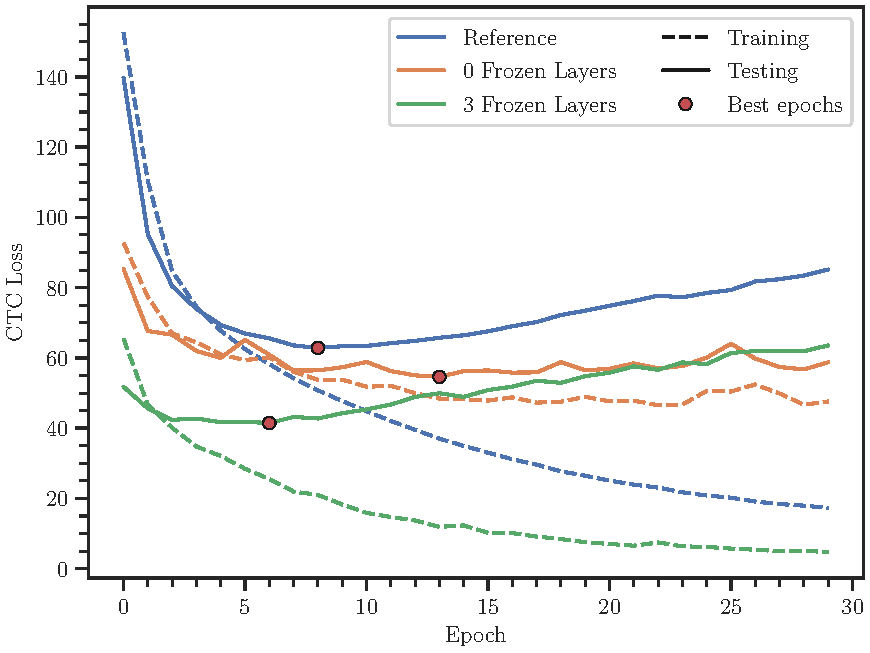
\includegraphics{3curves_de.pdf}
    \caption{Learning curves (German dataset): With and without transfer learning and layer freezing}
    \label{fig:3c}
\end{figure}

\begin{figure}[htbp]
    \centering
    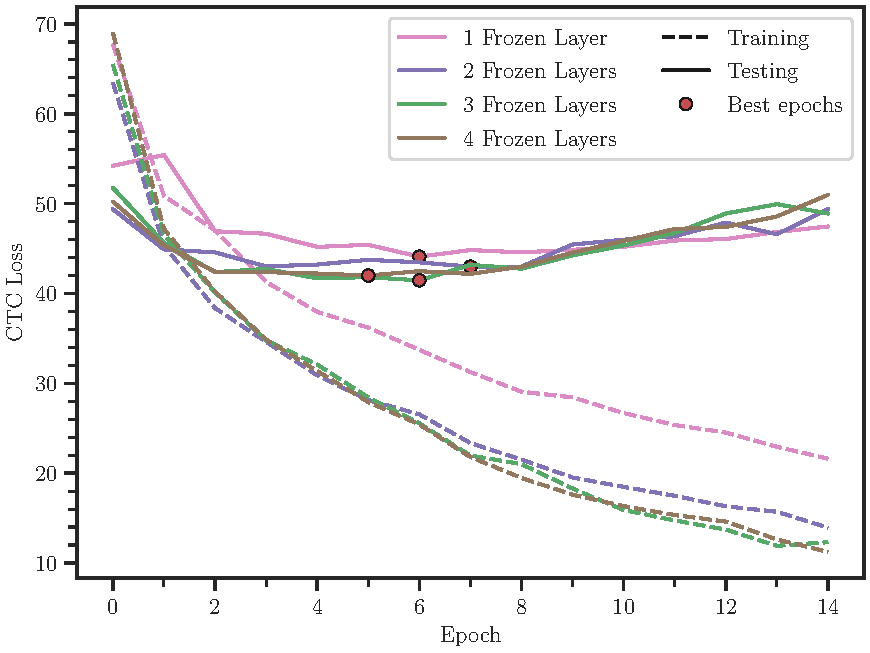
\includegraphics{4curves_de.pdf}
    \caption{Learning curves (German dataset): Comparison of freezing a different number of layers}
    \label{fig:4c}
\end{figure}

\begin{figure}[htbp]
    \centering
    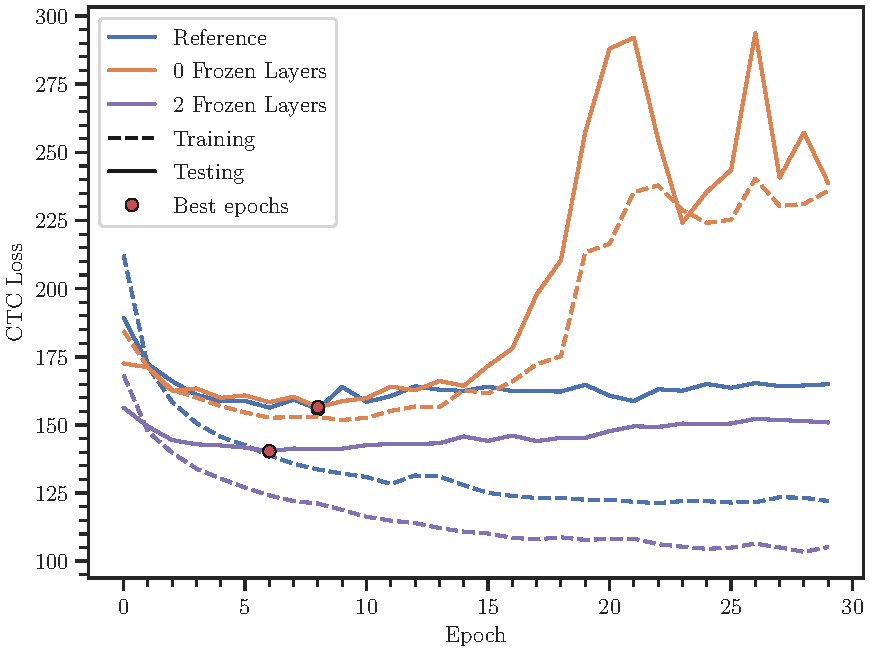
\includegraphics{3curves_ch.pdf}
    \caption{Learning curves (Swiss German dataset): With and without transfer learning and layer freezing}
    \label{fig:3ch}
\end{figure}

\begin{figure}[htbp]
    \centering
    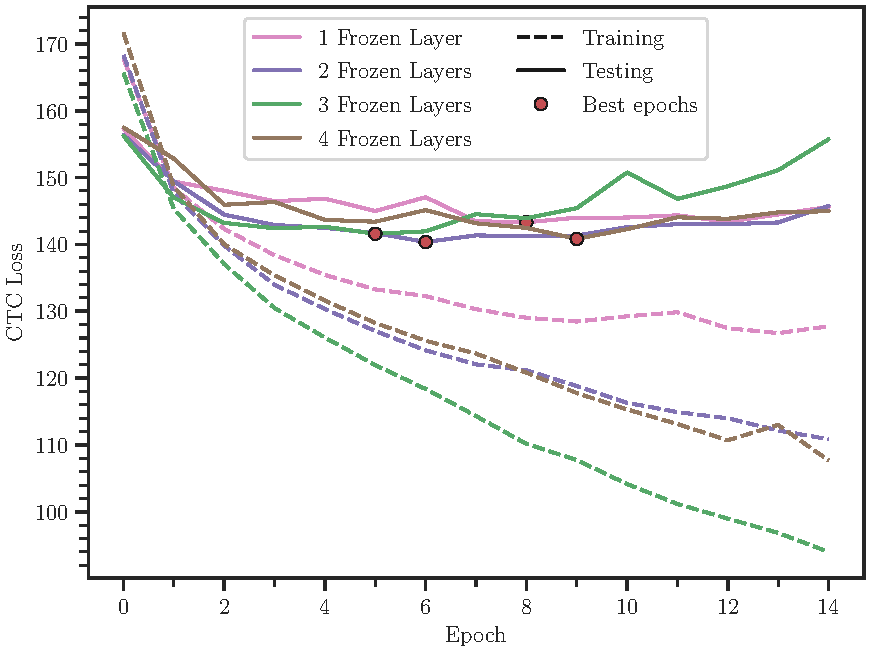
\includegraphics{4curves_ch.pdf}
    \caption{Learning curves (Swiss German dataset): Comparison of freezing a different number of layers}
    \label{fig:4ch}
\end{figure}

For both languages, the best results were achieved by the models with the first two to three layers frozen during training. It is notable however, that the other models that utilize layer freezing are not far off. The training curves look remarkably similar (see Figures \ref{fig:4c} and \ref{fig:4ch}). For both languages, all four models achieve much better results than the two models without layer freezing ("Reference" and "0 Frozen Layers"). The results seem to indicate that freezing the first layer brings the largest advantage in training, with diminishing returns on freezing the second and third layers. For German, additionally freezing the fifth layer slightly worsens the result. For Swiss German, the result slightly worsens when the third layer is frozen and stays almost constant when additionally freezing the fifth layer. Similar results were achieved by \textcite{DBLP:conf/lrec/ArdilaBDKMHMSTW20}, where freezing two or three layers also achieved the best transfer results for German, with a word error rate of 44\%. They also used DeepSpeech and a different version of the German Common Voice dataset.

The models with four frozen layers could only optimize the LSTM weights and the weights of the output layer. It is surprising that they still achieve good results. It might be interesting to see what happens when the LSTM layer is frozen as well. It is probable that with a larger dataset the benefits of freezing weights decrease and better results are achieved with freezing fewer or no layers. This might be the reason why with the larger German dataset the performance gets worse when freezing four instead of three layers, but not so with the smaller Swiss German dataset. For both languages it is evident that the transfer learning approach is promising.

\section{Further Research}
A next step might be to train these models with more training data and see if layer freezing is still beneficial. The chosen German speech dataset is not very large; \textcite{agarwal-zesch-2019-german} achieved a best result of 0.151 WER when training the model on a large dataset, in contrast to a result of 0.797 WER when training the same model on a very similar dataset to the one we used.

An interesting idea for further research is to use a different pretrained model than the English one. English seems to work alright for transferring to German, but it is possible that the lower level language features extracted by a model only trained for recognizing English speech are not sufficient for transferring to certain other languages. For example, when just transcribing speech there is no need for such a model to learn intonation features. This might be a problem when trying to transfer such a pretrained model to a tonal language like Mandarin or Thai. There might also be phonemes that don't exist or are very rare in English but abundant in other languages. 

% For these reasons one could try and build a new model that is trained on language data from many different languages, with the same task of transcribing speech to text. The model will not be good at this task, because it would have to learn all these languages at the same time and differentiate between them, which is not easy without a very large number of tunable parameters\footnote{A GPT-3-sized \parencite{brown2020language} model might be able to learn many languages simultaneously}. However, if trained correctly, it should at least extract the lower level features from these languages. This means that it should be possible to transfer this "bad" model to any language and get good results without large amounts of training data, when using layer freezing again. One might want to make the initial "bad" model much larger than DeepSpeech because it can be trained on large amounts of speech data from many languages. The size does not matter too much when transferring, because most of the weights would be frozen.

% To implement this idea, the DeepSpeech implementation used in this paper is not sufficient, because it does not support training on languages with different alphabet sizes at the same time. Instead, it might be possible to use a multitask learning approach, where the model is not only trained to output the correct character, but also the language of the current utterance. The predicted language can then be used to select the correct alphabet used for predicting the current character.

\section{Summary}
Transfer learning seems to be a powerful approach to train an automatic speech recognition system on a small dataset. The effects we saw when transferring DeepSpeech from English to German and from English to Swiss German were very similar: The results were not necessarily better than plain training when just initializing the parameters, but freezing only the first layer already improved the results dramatically. Freezing more layers improved the outcome even more, but with larger training datasets this might have adverse effects.

\section{Acknowledgements}
We want to thank Aashish Agarwal for valuable help in setting up DeepSpeech and for providing preprocessing scripts as well as the hyperparameters we used for training.

\printbibliography

\end{document}
